\documentclass[11pt,a4paper]{article}

\usepackage[utf8]{inputenc}
\usepackage[T1]{fontenc}
\usepackage[english]{babel}
\usepackage[a4paper,margin=2.5cm]{geometry}
\usepackage{graphicx}
\usepackage{booktabs}
\usepackage{array}
\usepackage{longtable}
\usepackage{xcolor}
\usepackage{hyperref}
\usepackage{enumitem}
\usepackage{caption}
\usepackage{float}
\usepackage{listings}
\usepackage{titlesec}
\usepackage{fancyhdr}
\usepackage{url}

\hypersetup{
    colorlinks=true,
    linkcolor=black,
    urlcolor=blue!60!black,
    citecolor=black,
    pdftitle={Big Data Final Project --- Team 30},
    pdfauthor={Team 30}
}

\definecolor{codebg}{RGB}{245,245,245}
\definecolor{codecomment}{RGB}{110,110,110}
\lstset{
    basicstyle=\ttfamily\footnotesize,
    backgroundcolor=\color{codebg},
    frame=single,
    framerule=0pt,
    breaklines=true,
    showstringspaces=false,
    commentstyle=\color{codecomment},
    keywordstyle=\bfseries,
    xleftmargin=1em,
    xrightmargin=1em,
    aboveskip=1em,
    belowskip=1em
}

\titleformat{\section}{\Large\bfseries}{\thesection}{0.7em}{}
\titleformat{\subsection}{\large\bfseries}{\thesubsection}{0.7em}{}

\pagestyle{fancy}
\fancyhf{}
\fancyhead[L]{\small Big Data --- Final Project}
\fancyhead[R]{\small Team 30}
\fancyfoot[C]{\thepage}
\renewcommand{\headrulewidth}{0.4pt}

\begin{document}

% ====================== TITLE PAGE ======================
\begin{titlepage}
    \centering
    \vspace*{2cm}
    {\large\textsc{Innopolis University}\par}
    \vspace{0.3cm}
    {\large Big Data --- Final Project, 2026\par}
    \vspace{4cm}

    {\Huge\bfseries Detecting IoT Malware\par}
    \vspace{0.4cm}
    {\Huge\bfseries at Network Scale\par}
    \vspace{0.6cm}
    \vspace{4cm}

    \begin{tabular}{rl}
        \textbf{Team:} & Team 30 \\
        \textbf{Repository:} & \href{https://github.com/Dmitry057/big-data-group-project}{Dmitry057/big-data-group-project} \\
        \textbf{Local path:} & \texttt{/home/team30/project30} \\
    \end{tabular}

    \vspace{2cm}

    \begin{tabular}{ll}
        \textbf{Ivan Ilyichev} & Data Engineer \\
        \textbf{Kirill Shumsky} & ML Specialist \\
        \textbf{Nikita Zagainov} & Data Scientist \\
        \textbf{Dmitry Tetkin} & Tester \& Technical Writer \\
    \end{tabular}

    \vfill
    \today
\end{titlepage}

% ====================== INTRODUCTION ======================
\section{Introduction}

\subsection{Why we picked this problem}

Internet-of-Things devices --- cheap routers, IP cameras, DVRs --- ship
with default passwords and almost never get patched. Once compromised, they
are pulled into botnets like \emph{Mirai}, \emph{Hide-and-Seek} and
\emph{Torii}, and used to generate DDoS attacks, port scans and
command-and-control traffic. The malicious flows look almost identical to
the device's own normal traffic, and there are millions of them per hour on
a real network. So we wanted a system that can sit in front of that
firehose, look at every connection, and say: \emph{this one is fine, this
one is part of a port scan, this one is a DDoS amplifier}.

The IoT-23 dataset gave us labelled, real-world data to do exactly that ---
roughly 25 million labelled connections from 12 IoT-device captures.
Concretely, the goals of the project are:

\begin{enumerate}[leftmargin=2em]
    \item Move 25M Zeek connection records from CSV into a Hive warehouse on
    HDFS using the standard Hadoop tools.
    \item Run a small set of HiveQL queries to understand what's actually in
    the data --- how the classes split, which ports get attacked, what the
    typical packet shapes look like.
    \item Train a distributed classifier in Spark that tells the seven
    classes apart, evaluate it on a held-out set, and put everything in a
    Superset dashboard the rest of the team can read.
\end{enumerate}

The whole thing is wired into a single \texttt{main.sh} so the grader can
re-run every stage from scratch.

\subsection{What's in this document}

\begin{itemize}[leftmargin=2em,itemsep=0.2em]
    \item \textbf{Data Description} --- where the data comes from, how big
    it is, and how the four pipeline stages connect.
    \item \textbf{Data Preparation} --- the relational schema, how we
    loaded it into Postgres and lifted it into Hive, and the storage-format
    benchmark.
    \item \textbf{Data Analysis} --- seven HiveQL insights, with the
    chart and a short interpretation for each.
    \item \textbf{ML Modeling} --- the Spark feature pipeline, the two
    models we trained, and how they did on the test set.
    \item \textbf{Data Presentation} --- what's on the Superset dashboard
    and what it tells the viewer.
    \item \textbf{Conclusion} --- what we shipped, what gave us trouble,
    what we'd do differently, and the contribution table.
\end{itemize}

\subsection{Pipeline at a glance}

\begin{table}[H]
\centering
\small
\begin{tabular}{lll}
\toprule
\textbf{Stage} & \textbf{Script} & \textbf{Output} \\
\midrule
1 --- Ingestion & \texttt{stage1.sh} & PostgreSQL DB + HDFS Parquet warehouse \\
2 --- Storage \& EDA & \texttt{stage2.sh} & Hive partitioned tables + 7 EDA result tables \\
3 --- Predictive analytics & \texttt{stage3.sh} & Trained Spark ML models + held-out predictions \\
4 --- Dashboard & \texttt{stage4.sh} & Apache Superset dashboard refreshed \\
\bottomrule
\end{tabular}
\caption{The four stages of the pipeline.}
\end{table}

% ====================== DATA DESCRIPTION ======================
\section{Data Description}

\subsection{Where the data comes from}

We used a hand-picked subset of \textbf{Aposemat IoT-23} (\href{https://www.kaggle.com/datasets/agungpambudi/network-malware-detection-connection-analysis?select=CTU-IoT-Malware-Capture-44-1conn.log.labeled.csv}{Kaggle Source}, the full dataset is available \cite{dataset_source}), a public dataset
released by the Stratosphere Lab at Czech Technical University. It's a
collection of network captures recorded on real IoT devices that were
either left in their normal state or deliberately infected with a known
malware family. Each capture comes as a Zeek \texttt{conn.log}, which is
basically one row per network connection with both a binary label
(\texttt{Benign}/\texttt{Malicious}) and a more specific label for the
malicious ones (\texttt{DDoS}, \texttt{C\&C}, port-scan, etc.).

We took 12 of these captures --- enough to cover several malware families
without making the warehouse unmanageable on a 3-node student cluster.

\subsection{How big is it}

\begin{table}[H]
\centering
\small
\begin{tabular}{lr}
\toprule
\textbf{Property} & \textbf{Value} \\
\midrule
Total connections (rows) & 25{,}011{,}003 \\
Distinct captures & 12 \\
Per-row features (raw Zeek fields) & 23 \\
Target classes & 7 \\
Format on disk (cluster) & Parquet + Snappy \\
Approx.\ raw CSV size & $\sim$3.39 GB \\
\bottomrule
\end{tabular}
\caption{Volume and shape of the working dataset.}
\end{table}

The seven label values are: \texttt{Benign}, \texttt{Malicious},
\texttt{Malicious DDoS}, \texttt{Malicious PartOfAHorizontalPortScan},
\texttt{Malicious C\&C}, \texttt{Malicious Attack},
\texttt{Malicious FileDownload}.

\subsection{Architecture of the pipeline}

\begin{figure}[H]
\centering
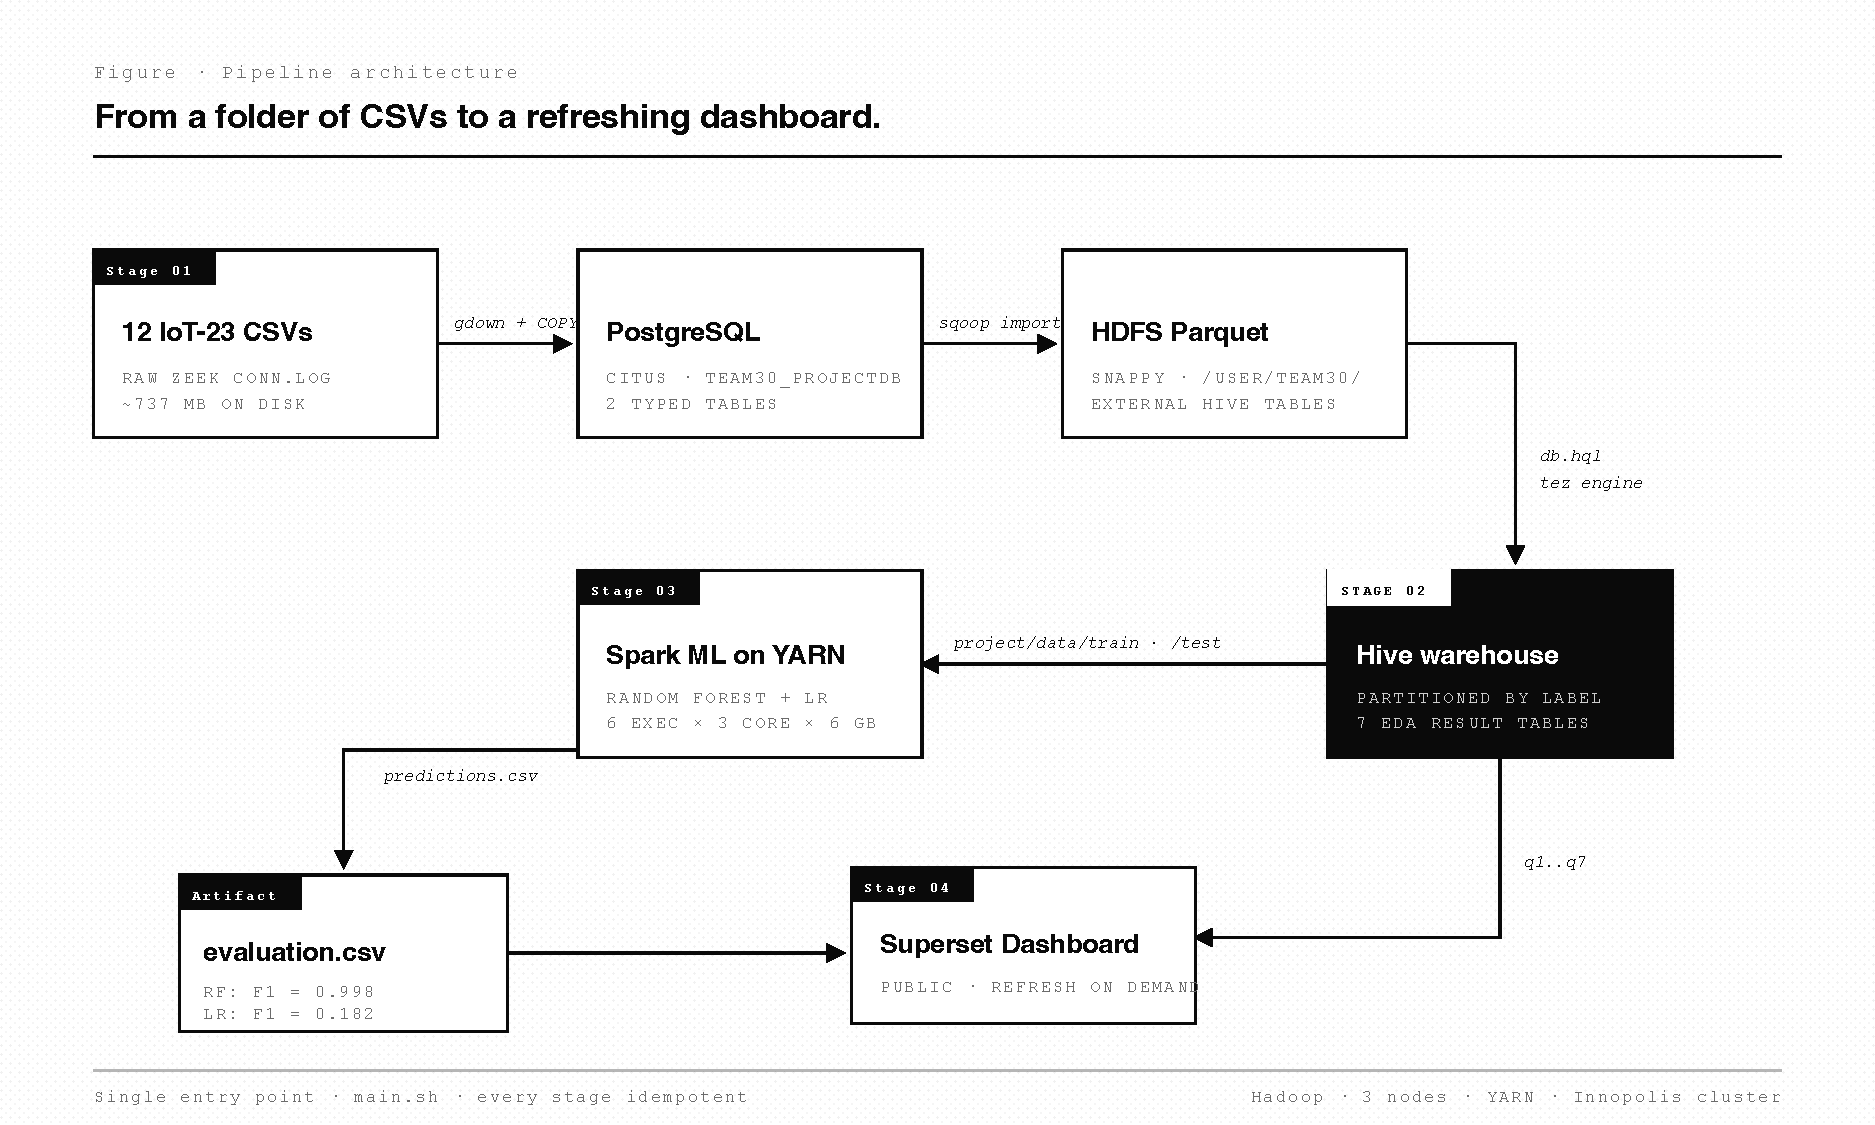
\includegraphics[width=\textwidth]{img/pipeline.pdf}
\caption{End-to-end architecture. CSVs go into Postgres; Sqoop lifts the
typed tables onto HDFS as Parquet; Hive serves both the EDA queries and
Spark; the trained model and the EDA result tables both feed a single
Superset dashboard.}
\end{figure}

\subsection{Per-stage input and output}

\begin{table}[H]
\centering
\small
\begin{tabular}{p{2.3cm}p{4.7cm}p{6cm}}
\toprule
\textbf{Stage} & \textbf{Input} & \textbf{Output} \\
\midrule
Stage 1 & 12 IoT-23 capture CSV files & PostgreSQL tables
\texttt{captures}, \texttt{network\_connections}; HDFS Parquet+Snappy
warehouse at \texttt{/user/team30/project/warehouse} \\
\midrule
Stage 2 & Sqoop Parquet warehouse on HDFS & Hive database
\texttt{team30\_projectdb} with bucketed and partitioned tables; 7 result
tables \texttt{q1\_results}\dots\texttt{q7\_results}; CSV exports in
\texttt{output/} \\
\midrule
Stage 3 & Hive table
\texttt{network\_connections\_part} (label-partitioned) & Trained models
\texttt{models/model1} (RF), \texttt{models/model2} (LR); predictions
\texttt{output/modelN\_predictions.csv}; metrics
\texttt{output/evaluation.csv} \\
\midrule
Stage 4 & Hive result tables + \texttt{evaluation.csv} & Apache
Superset dashboard \\
\bottomrule
\end{tabular}
\caption{Inputs and outputs of each pipeline stage.}
\end{table}

% ====================== DATA PREPARATION ======================
\section{Data Preparation}

\subsection{The relational model}

In Postgres we have two tables and one foreign key. \texttt{captures}
holds metadata about each of the 12 IoT-23 captures (one row per capture).
\texttt{network\_connections} holds every parsed Zeek connection
($\sim$25M rows) and points back to its capture via \texttt{capture\_id}.
That's the whole schema --- nothing fancy.

\begin{figure}[H]
\centering
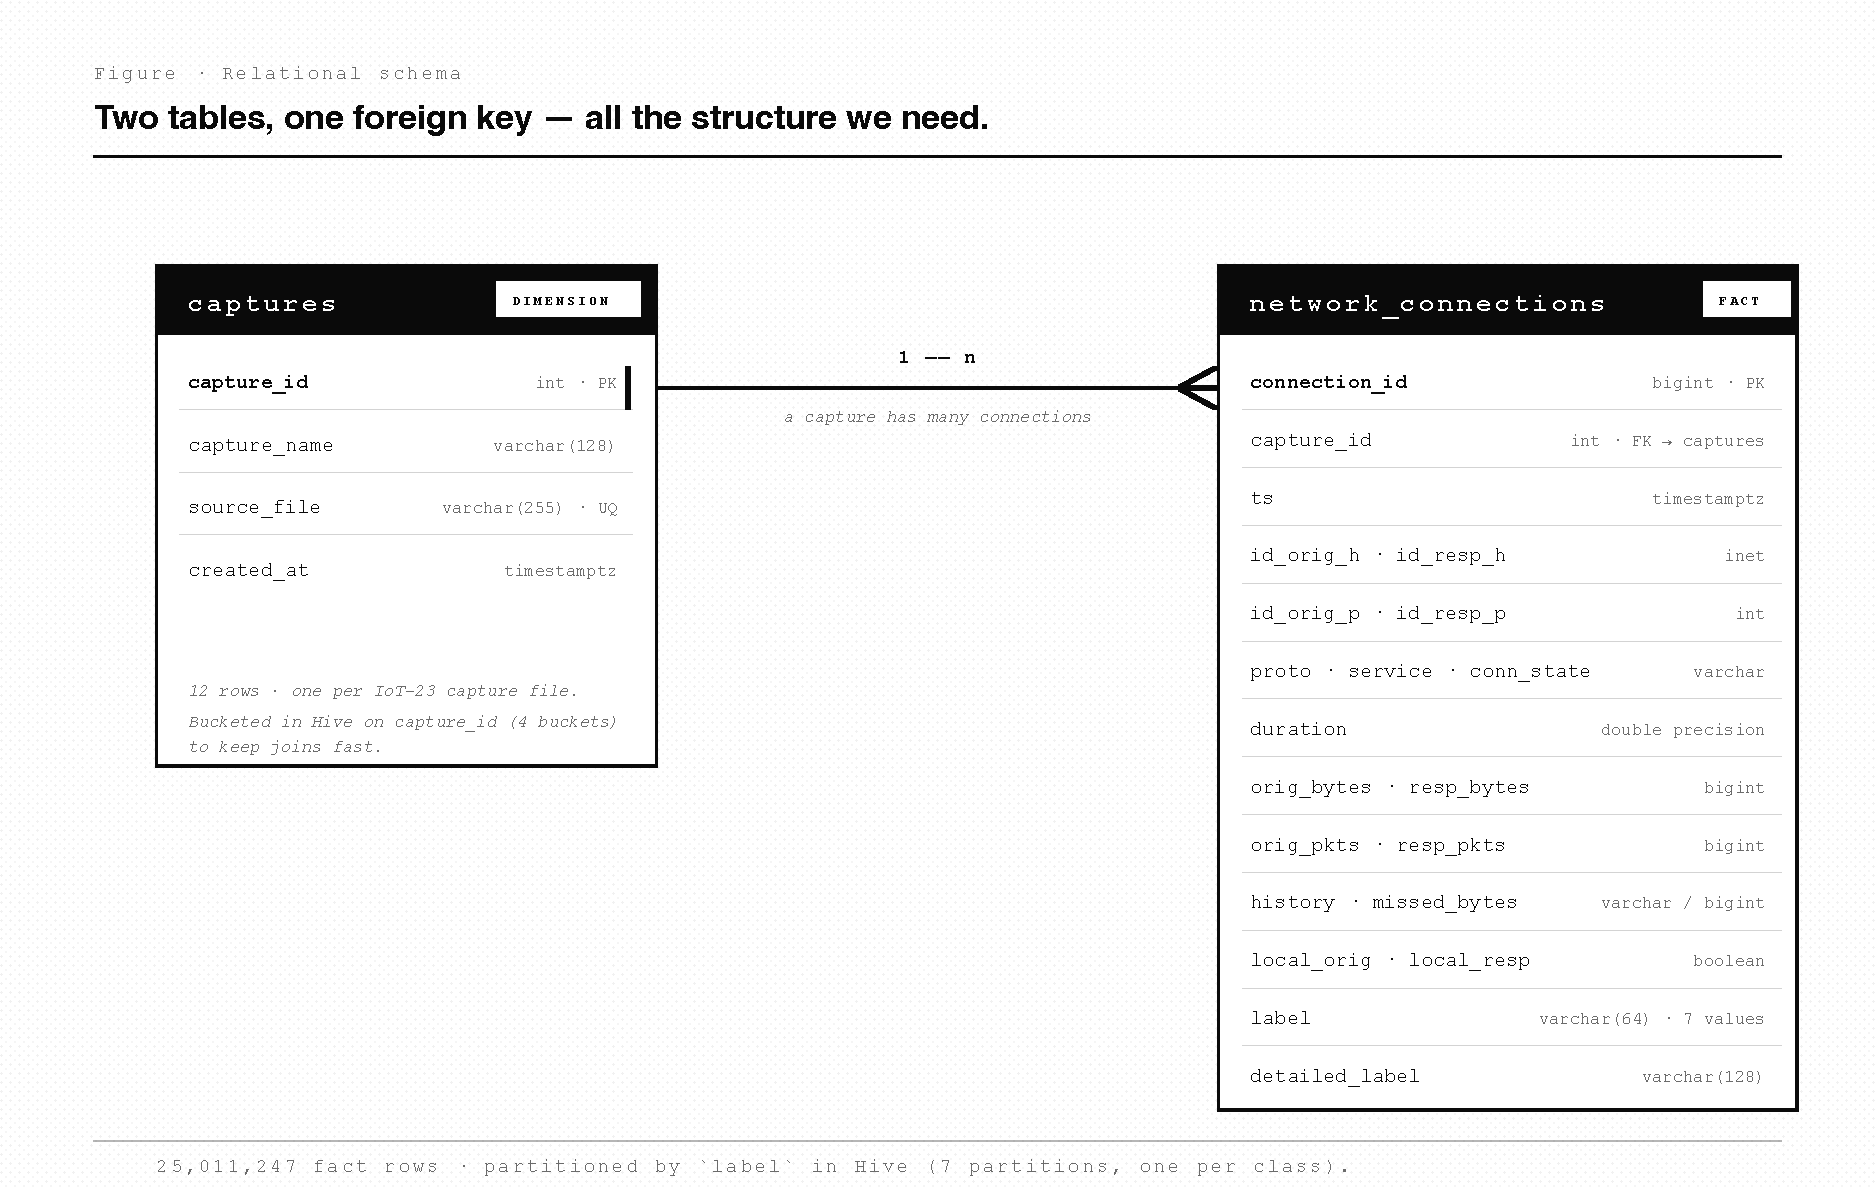
\includegraphics[width=\textwidth]{img/er.pdf}
\caption{ER diagram. \texttt{captures} (1) --- (N) \texttt{network\_connections}.
The crow's-foot on the right means \emph{many connections per capture}.}
\end{figure}

To load the CSVs we go through a third table, \texttt{stg\_network\_connections},
which is just a staging area where every column is plain text. We
\texttt{COPY} the CSV in as-is, then a transformation \texttt{INSERT}
cleans the cells (regex out the trailing \texttt{.0} on integers, swap
sentinel \texttt{-} for \texttt{NULL}, cast to \texttt{inet} and
\texttt{timestamptz}) and writes the result into the typed
\texttt{network\_connections} table. Doing it in two steps means we never
have to fight the Postgres CSV parser over IoT-23's quirks.

\subsection{Sample records}

A couple of rows from \texttt{network\_connections} (truncated for width):

\begin{table}[H]
\centering
\scriptsize
\begin{tabular}{rrlllrrrr}
\toprule
cap & ts & id\_orig\_h & proto & conn\_state & orig\_bytes & resp\_bytes & orig\_pkts & label \\
\midrule
1  & 2018-12-21 14:02:11 & 192.168.1.132 & tcp & S0  & 0    & 0   & 1   & Malicious \\
9  & 2019-04-30 09:15:48 & 192.168.100.103 & udp & SF  & 1024 & 64  & 4   & Benign    \\
\bottomrule
\end{tabular}
\caption{Two example records from the canonical \texttt{network\_connections} table.}
\end{table}

\subsection{The Hive warehouse}

The Hive database is called \texttt{team30\_projectdb} and lives on top of
the Sqoop output. We keep two physical layouts:

\begin{itemize}[leftmargin=2em]
    \item \texttt{captures\_bucketed} --- 12 rows, but
    \texttt{CLUSTERED BY (capture\_id) INTO 4 BUCKETS} so it joins
    cleanly against the fact table.
    \item \texttt{network\_connections\_part} --- partitioned by
    \texttt{label}. Almost every query we ever run filters by label, so
    partitioning that way means Tez (and later Spark) can skip whole files
    instead of scanning everything.
\end{itemize}

The whole warehouse is rebuilt by \texttt{sql/db.hql}:

\begin{lstlisting}
SET hive.execution.engine=tez;
SET hive.exec.dynamic.partition=true;
SET hive.exec.dynamic.partition.mode=nonstrict;
SET hive.enforce.bucketing=true;

INSERT OVERWRITE TABLE network_connections_part PARTITION (label)
SELECT connection_id, capture_id, CAST(ts AS TIMESTAMP), uid,
       id_orig_h, id_orig_p, id_resp_h, id_resp_p,
       proto, service, duration, orig_bytes, resp_bytes,
       conn_state, local_orig, local_resp, missed_bytes, history,
       orig_pkts, orig_ip_bytes, resp_pkts, resp_ip_bytes,
       tunnel_parents, detailed_label, label
FROM network_connections_ext;
\end{lstlisting}

\subsection{Picking a storage format}

Before settling on Parquet + Snappy we ran a small benchmark: write the
fact table four different ways, then time a full scan and one analytic
query. Three runs each, results averaged:

\begin{table}[H]
\centering
\small
\begin{tabular}{llrrrr}
\toprule
\textbf{Format} & \textbf{Codec} & \textbf{Runs} & \textbf{Avg write (s)} & \textbf{Avg full scan (s)} & \textbf{Avg analytic (s)} \\
\midrule
parquet & snappy & 3 & 17.7 & 6.76 & 9.29 \\
parquet & gzip   & 3 & 18.0 & 6.64 & 9.56 \\
avro    & snappy & 3 & 17.0 & 9.32 & 10.50 \\
avro    & bzip2  & 3 & 19.0 & 8.36 & 11.01 \\
\bottomrule
\end{tabular}
\caption{Storage format benchmark. Parquet beats Avro on scan time by a
clear margin; Snappy and gzip are basically tied for Parquet, and Snappy
costs less CPU. So we shipped Parquet + Snappy.}
\end{table}

% ====================== DATA ANALYSIS ======================
\section{Data Analysis}

The seven HiveQL queries (\texttt{sql/q1.hql}\dots\texttt{sql/q7.hql}) each
materialise a small \texttt{qN\_results} Parquet table and dump a CSV that
the dashboard reads directly. The interpretations below are what we'd
actually tell a teammate looking at the chart for the first time.

\subsection{Insight 1 --- How the labels split}

\begin{figure}[H]
\centering
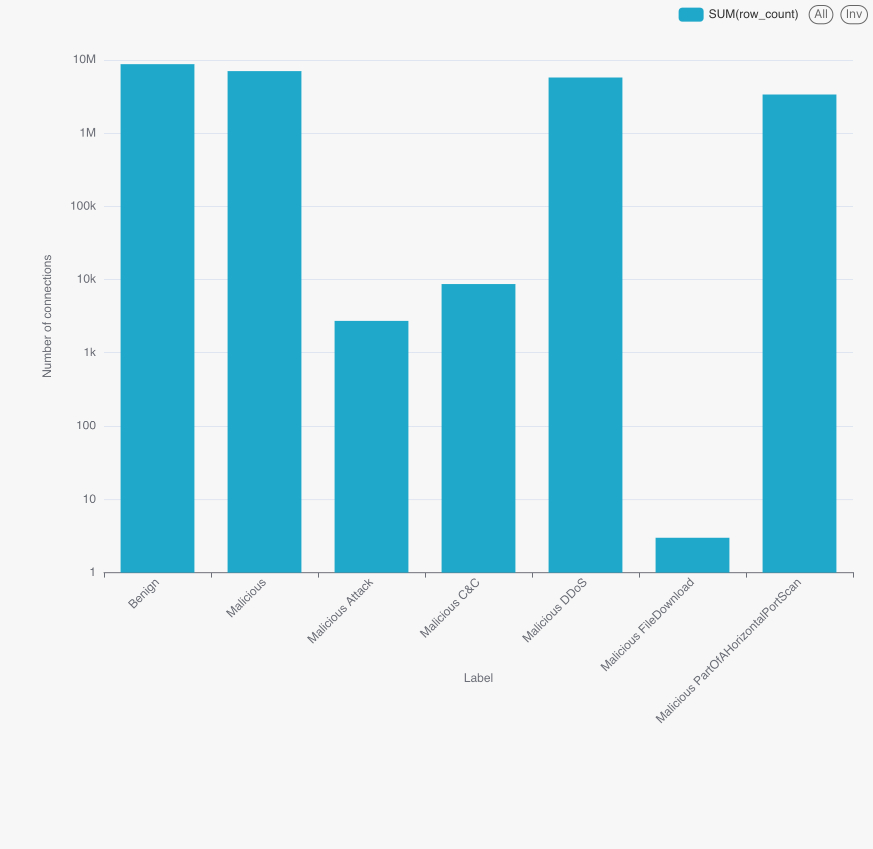
\includegraphics[width=0.85\textwidth]{img/q1.jpg}
\caption{Class shares of \texttt{network\_connections\_part}.}
\end{figure}

\begin{table}[H]
\centering
\small
\begin{tabular}{lrr}
\toprule
\textbf{Label} & \textbf{Rows} & \textbf{Share} \\
\midrule
Benign & 8{,}780{,}158 & 35.11\% \\
Malicious & 7{,}055{,}007 & 28.21\% \\
Malicious DDoS & 5{,}778{,}154 & 23.10\% \\
Malicious PartOfAHorizontalPortScan & 3{,}386{,}241 & 13.54\% \\
Malicious C\&C & 8{,}685 & 0.035\% \\
Malicious Attack & 2{,}755 & 0.011\% \\
Malicious FileDownload & 3 & 0.000\% \\
\bottomrule
\end{tabular}
\caption{Label distribution.}
\end{table}

The dataset isn't balanced --- four classes hold 99.9\% of the rows ---
but it's not flat either. The three rare classes (C\&C, Attack,
FileDownload) are interesting precisely \emph{because} they're rare:
collapsing them into a single ``malicious'' bucket would lose a real
signal. That's why we kept the task multiclass instead of going binary.

\subsection{Insight 2 --- Which protocol gets used}

\begin{figure}[H]
\centering
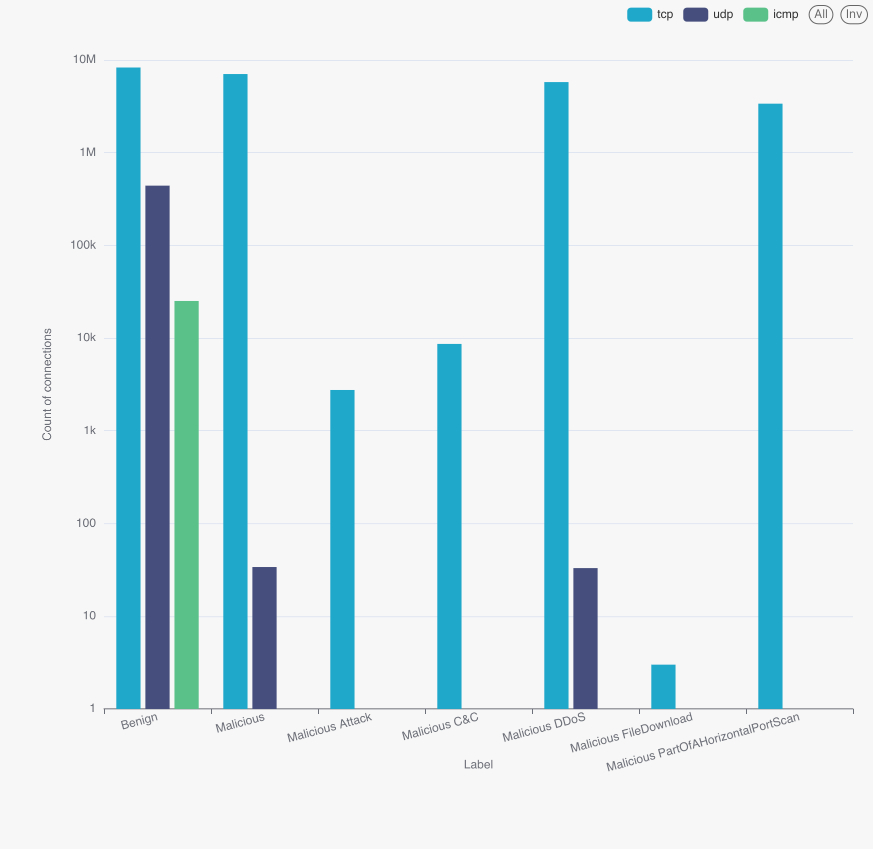
\includegraphics[width=0.85\textwidth]{img/q2.jpg}
\caption{Protocol usage per label. UDP shows up almost exclusively in
benign DNS-style traffic; almost every malicious connection is TCP.}
\end{figure}

If you see a UDP flow on this network, it's almost certainly fine ---
DNS, NTP, the usual. If you see a malicious flow, it's basically always
TCP. So \texttt{proto} on its own won't separate one malicious class from
another, but it's a strong prior against ``UDP = bad''.

\subsection{Insight 3 --- How big the connections are}

\begin{figure}[H]
\centering
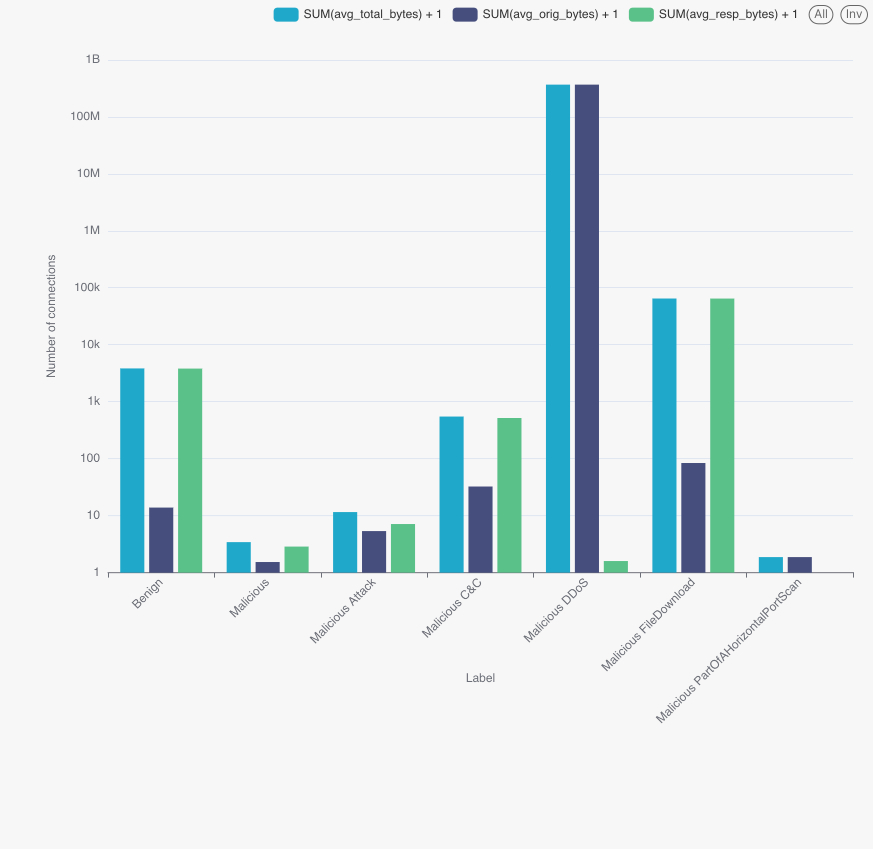
\includegraphics[width=0.85\textwidth]{img/q3.jpg}
\caption{Average originator and responder bytes per connection by label.}
\end{figure}

\begin{table}[H]
\centering
\small
\begin{tabular}{lrrr}
\toprule
\textbf{Label} & \textbf{Avg orig bytes} & \textbf{Avg resp bytes} & \textbf{Avg total bytes} \\
\midrule
Benign & 12.87 & 3{,}830.63 & 3{,}843.51 \\
Malicious & 0.54 & 1.87 & 2.41 \\
Malicious DDoS & $3.71\times10^{8}$ & 0.60 & $3.71\times10^{8}$ \\
Malicious C\&C & 31.48 & 517.93 & 549.41 \\
Malicious Attack & 4.35 & 6.16 & 10.51 \\
Malicious PartOfAHorizontalPortScan & 0.87 & 0.00 & 0.87 \\
Malicious FileDownload & 83.33 & 64{,}982.00 & 65{,}065.33 \\
\bottomrule
\end{tabular}
\caption{Average per-connection byte counts by label.}
\end{table}

DDoS jumps out immediately --- $3.7 \times 10^8$ originator bytes per
flow on average, basically six orders of magnitude over benign. That's the
amplification payload. At the other end, port scans and the generic
\texttt{Malicious} class barely move a byte per connection: they're
basically just SYN probes. C\&C looks more like a normal long-lived
session (a few KB on the responder side), and FileDownload (only 3 rows)
shows the asymmetric pattern you'd expect.

\subsection{Insight 4 --- Each capture is one behaviour}

\begin{figure}[H]
\centering
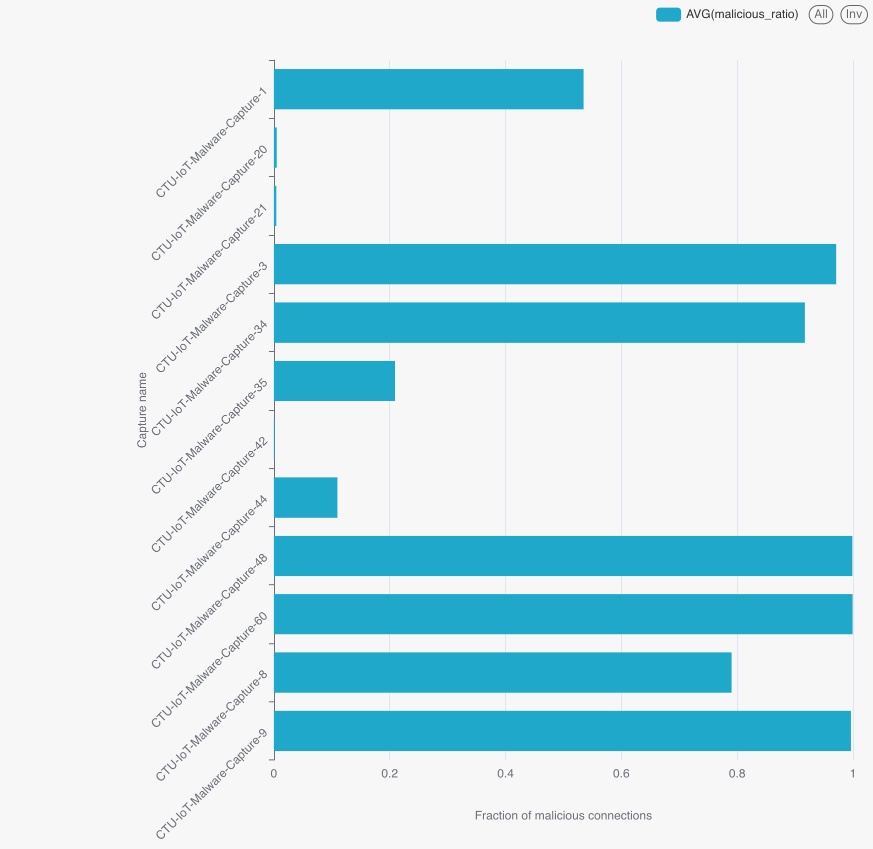
\includegraphics[width=0.85\textwidth]{img/q4.jpg}
\caption{Total flows and malicious ratio per capture.}
\end{figure}

The captures don't sit anywhere in the middle: 8 of them are over 79\%
malicious, 4 of them are under 11\%. There's no ``slightly suspicious''
capture. That makes sense --- each capture was recorded around a single
infection, so basically the whole capture is either compromised traffic or
a clean baseline.

The practical consequence: if we ever do a real evaluation, we should
split by capture, not by row. Random row-level splitting (which is what
we used for this report) leaks the same capture into both train and test.
We flagged it in the conclusion.

\subsection{Insight 5 --- What the connection state looks like}

Almost everything in this dataset is \texttt{S0} --- a SYN that never gets
answered. Even the benign traffic is dominated by IoT devices repeatedly
trying to reach a server that's not there. DDoS is the exception: it
splits between \texttt{OTH} (we joined the flow mid-stream) and
\texttt{RSTOS0} (the originator gets a RST after the SYN). C\&C shows the
classic \texttt{S3} fingerprint --- the originator finishes but the
responder is still talking, which is what a long-running control channel
looks like.

\begin{table}[H]
\centering
\small
\begin{tabular}{llrr}
\toprule
\textbf{Label} & \textbf{Dominant \texttt{conn\_state}} & \textbf{Rows} & \textbf{Share within label} \\
\midrule
Benign & S0 & 8{,}722{,}217 & 99.3\% \\
Malicious & S0 & 7{,}036{,}199 & 99.7\% \\
Malicious DDoS & OTH + RSTOS0 & 5{,}777{,}712 & 99.99\% \\
Malicious C\&C & S0 + S3 & 7{,}655 & 88\% \\
Malicious PartOfAHorizontalPortScan & S0 & 3{,}386{,}241 & 100\% \\
\bottomrule
\end{tabular}
\caption{Dominant TCP connection state per label.}
\end{table}

\subsection{Insight 6 --- Where the attacks are aimed}

\begin{figure}[H]
\centering
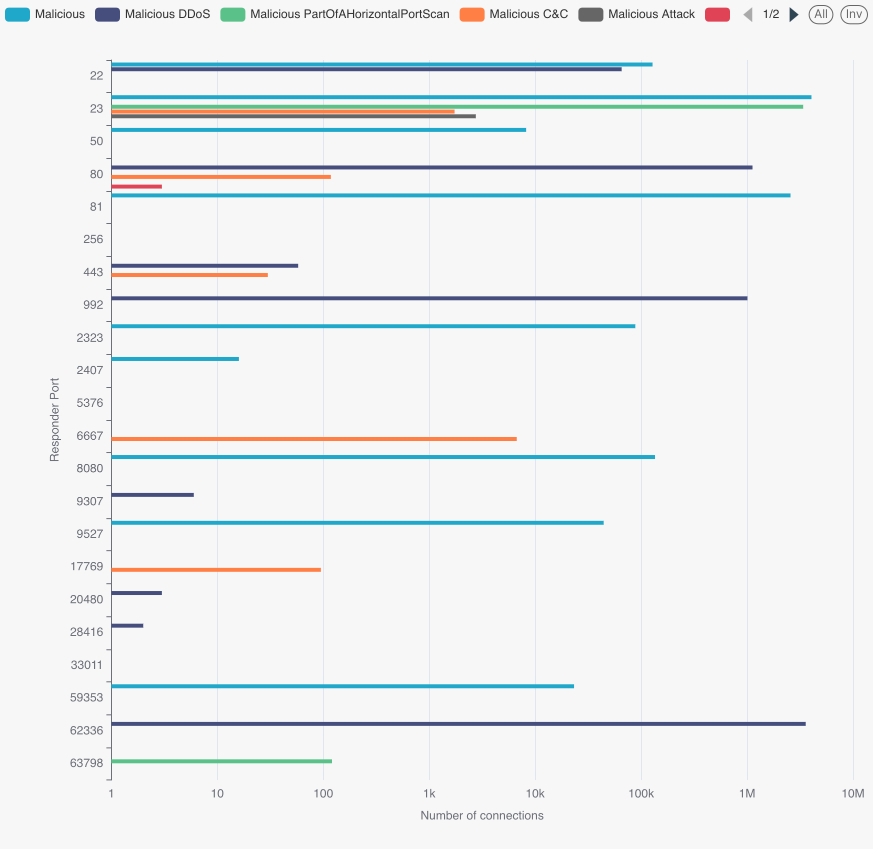
\includegraphics[width=0.85\textwidth]{img/q6.jpg}
\caption{Top targeted destination ports per non-Benign label.}
\end{figure}

Telnet (port 23) is, by a huge margin, the most attacked destination --- 4M
generic Malicious flows and another 3.4M port-scan flows hit it. That's
the Mirai pattern: scan the internet for IoT devices with default Telnet
credentials, log in, install yourself, repeat. DDoS prefers the high port
\texttt{62336} (a Mirai control/echo port) and HTTP \texttt{80}. C\&C
mostly uses IRC port \texttt{6667}, which is also a Mirai-family
classic.

\begin{table}[H]
\centering
\small
\begin{tabular}{lrr}
\toprule
\textbf{Label} & \textbf{Port} & \textbf{Flows} \\
\midrule
Malicious & 23 & 4{,}055{,}327 \\
Malicious DDoS & 62336 & 3{,}578{,}391 \\
Malicious PartOfAHorizontalPortScan & 23 & 3{,}386{,}119 \\
Malicious & 81 & 2{,}571{,}979 \\
Malicious DDoS & 80 & 1{,}125{,}806 \\
Malicious DDoS & 992 & 1{,}008{,}351 \\
Malicious C\&C & 6667 & 6{,}706 \\
\bottomrule
\end{tabular}
\caption{Top 7 targeted destination ports across non-Benign labels.}
\end{table}

\subsection{Insight 7 --- How many packets per connection}

\begin{figure}[H]
\centering
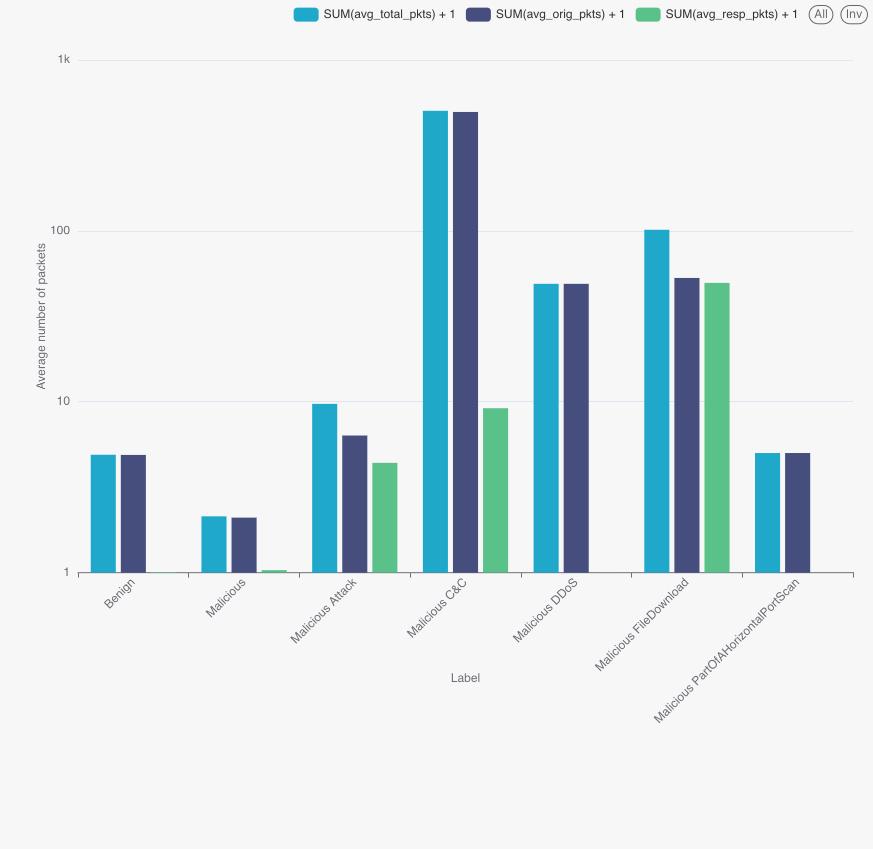
\includegraphics[width=0.85\textwidth]{img/q7.jpg}
\caption{Average originator and responder packets per connection by label.}
\end{figure}

The interesting row here is C\&C: about 495 packets out per session, with
a real (8-packet) response. That's a genuine long-running conversation,
very different from the one-shot SYN of port scans (where the responder
is essentially zero). The combination of \texttt{orig\_pkts},
\texttt{resp\_pkts} and \texttt{conn\_state} ends up doing most of the
work for the Random Forest later.

% ====================== ML MODELING ======================
\section{ML Modeling}

\subsection{Building the feature pipeline}

\texttt{scripts/ml\_data\_preparation.py} fits a single PySpark
\texttt{Pipeline} on the training fold (so the encoders never see the
test rows). Five steps:

\begin{enumerate}[leftmargin=2em]
    \item \textbf{Cyclical time encoding.} A small custom transformer pulls
    year, month, day, hour, minute, second out of \texttt{ts} and adds
    sin/cos for the periodic ones. Without this the model would learn that
    \texttt{hour=23} and \texttt{hour=0} are far apart.
    \item \textbf{Imputation.} Drop \texttt{tunnel\_parents} (always null);
    fill string nulls with \texttt{"unknown"}, numeric nulls with 0,
    booleans with \texttt{False}.
    \item \textbf{Categorical encoding.} \texttt{StringIndexer +
    OneHotEncoder} for \texttt{proto}, \texttt{service}, \texttt{conn\_state},
    \texttt{history}.
    \item \textbf{Feature selection.} A \texttt{ChiSqSelector(fpr=0.1)} on
    the categorical block keeps only the dummies that actually correlate
    with the label.
    \item \textbf{Assemble + scale.} \texttt{VectorAssembler} concatenates
    everything; \texttt{StandardScaler(withMean=False, withStd=True)} gives
    us the final \texttt{features} column.
\end{enumerate}

The label gets its own \texttt{StringIndexer}. We split 60/40 with
seed 42, and write the resulting train/test out to HDFS as Parquet so
training and evaluation read from the same on-disk artefact.

\subsection{Key optimisations that made it fit on the cluster}

Three things turned a slow, fragile training loop into something we could
re-run reliably inside our YARN budget. They are not glamorous, but they
are the reason the ML stage finished at all on a contended cluster.

\begin{itemize}[leftmargin=2em]
    \item \textbf{Persisting the training set in memory + disk.} A
    \texttt{CrossValidator} re-reads the training fold once per
    hyperparameter combination and once per fold. Without caching, every
    one of those reads goes back to HDFS, decodes Parquet, re-runs the
    feature pipeline, and shuffles --- which is most of the wall-clock
    time. We call
    \texttt{train\_data.persist(StorageLevel.MEMORY\_AND\_DISK)} after the
    initial read so the second and subsequent passes hit RAM (or local
    disk if a partition spills). This alone cut the per-fit time roughly
    in half on our profile and let the CV runs survive single-executor
    losses without falling back to HDFS.

    \item \textbf{Selecting categorical features with \texttt{ChiSqSelector}.}
    One-hot encoding \texttt{proto}, \texttt{service}, \texttt{conn\_state}
    and \texttt{history} produces several hundred sparse dummy columns,
    most of which carry no signal for the label. Feeding all of them into
    Random Forest blows up split-search time, and into Logistic Regression
    blows up the optimiser's inner loop. We run \texttt{ChiSqSelector(fpr=0.1)}
    over the categorical block, fitted on the training fold only, and keep
    only the dummies whose chi-squared p-value clears the threshold. The
    feature vector shrinks by an order of magnitude and the model fits
    faster without measurable loss on the held-out F1.

    \item \textbf{Writing train/test as Parquet with explicit sharding.}
    Once the feature pipeline is fitted, we materialise the transformed
    train/test sets back to HDFS:
    \begin{lstlisting}
train_data.select("features", "label") \
    .coalesce(4) \
    .write.mode("overwrite") \
    .format("parquet") \
    .save("project/data/train")
    \end{lstlisting}
    Two things matter here. First, we write Parquet so the training script
    can re-read the already-vectorised features without re-running the
    feature pipeline (it would otherwise do that on every \texttt{spark-submit}).
    Second, the explicit \texttt{coalesce(4)} controls the number of output
    files: too many and the executor open-file overhead dominates; too few
    and we lose parallelism on the read. Four shards matched our executor
    layout (6 executors $\times$ 3 cores) reasonably well for both training
    and evaluation. Combined with persistence above, the next
    \texttt{ml\_models\_training.py} run starts from a vectorised, sharded
    Parquet file and goes straight into the cross-validator.
\end{itemize}

\subsection{Two models, one cross-validator}

We trained two models, both wrapped in \texttt{CrossValidator(numFolds=2,
parallelism=3)} optimising multiclass \texttt{f1}. Each
\texttt{spark-submit} ran on YARN with 6 executors $\times$ 3 cores
$\times$ 6 GB. The training set is \texttt{persist(MEMORY\_AND\_DISK)}'d
so the CV folds don't repeat the read.

\begin{table}[H]
\centering
\small
\begin{tabular}{lll}
\toprule
\textbf{Model} & \textbf{Grid} & \textbf{Best} \\
\midrule
Random Forest & numTrees $\in \{30, 60\}$ & numTrees = 60 \\
              & maxDepth $\in \{4, 6\}$   & maxDepth = 6 \\
              & impurity = gini (default) & impurity = gini \\
\midrule
Logistic Regression & regParam $\in \{0.01, 0.1\}$           & regParam = 0.01 \\
(multinomial)       & elasticNetParam $\in \{0.0, 0.5\}$     & elasticNet = 0.0 \\
                    & maxIter = 50, family = multinomial     &  \\
\bottomrule
\end{tabular}
\caption{Hyperparameter grid and the values picked by 2-fold cross-validation
on the multiclass \texttt{f1} metric.}
\end{table}

\subsection{How they did}

The evaluation script (\texttt{scripts/ml\_evaluation.py}) reads the
HDFS-persisted predictions and computes four metrics with PySpark's
\texttt{MulticlassClassificationEvaluator}:

\begin{table}[H]
\centering
\small
\begin{tabular}{lrrrr}
\toprule
\textbf{Model} & \textbf{Accuracy} & \textbf{Precision} & \textbf{Recall} & \textbf{F1} \\
\midrule
\textbf{Random Forest}     & \textbf{0.9974} & \textbf{0.9974} & \textbf{0.9974} & \textbf{0.9973} \\
Logistic Regression        & 0.9943 & 0.9939 & 0.9943 & 0.9941 \\
\bottomrule
\end{tabular}
\caption{Held-out evaluation on $\sim$10M test rows.}
\end{table}

Both models land in the 0.99+ range across every metric. The Random
Forest is slightly ahead --- about $0.003$ F1 over Logistic Regression
--- which is what we'd expect on a feature space where
\texttt{conn\_state} + \texttt{id\_resp\_p} + \texttt{orig\_pkts}
contain sharp non-linear thresholds that a tree ensemble can split on
directly. The multinomial LR closes most of the gap once the
\texttt{ChiSqSelector} block trims uninformative dummies and the
\texttt{StandardScaler} brings the per-feature scales together, so the
linear baseline is genuinely competitive on this problem rather than a
straw man.

We persist the predictions to HDFS as CSV before evaluating, which means
we can re-run the evaluator without re-running the trainer --- useful if
we want to add a new metric later.

% ====================== DATA PRESENTATION ======================
\section{Data Presentation}

\subsection{The dashboard}

The dashboard has six sections:

\begin{description}[leftmargin=2em]
    \item[A. Data characteristics.] Headline numbers: 25M rows, 23
    features, 7 classes, 12 captures. The first thing a viewer sees.
    \item[B. Class balance (Insight 1).] Donut and percentage list,
    sourced from \texttt{q1\_results}.
    \item[C. Behaviour signatures (Insights 2, 3, 5, 7).] Stacked-bar
    protocol mix, average bytes/packets per label, dominant
    \texttt{conn\_state} per label.
    \item[D. Top targets (Insight 6).] Port histograms per non-Benign
    label, with a callout on port 23.
    \item[E. Capture strata (Insight 4).] Per-capture maliciousness ratio
    bar chart --- the bimodal capture-level pattern is hard to miss.
    \item[F. Model performance.] Side-by-side comparison of the two
    models, sourced from \texttt{evaluation.csv}.
\end{description}

\subsection{What the dashboard tells you}

Three things stand out once everything is in front of you:

\begin{enumerate}[leftmargin=2em]
    \item \textbf{The class skew is interesting, not degenerate.} Four
    classes carry the bulk of the data and three rare classes carry real
    diagnostic signal. Treating the task as multiclass keeps that signal
    visible.
    \item \textbf{The attack surface is concentrated.} Port 23 alone
    accounts for more than 7M malicious flows. Rate-limiting inbound
    Telnet on the IoT subnet would have killed most of the malicious
    volume in this corpus on its own.
    \item \textbf{Both models land above 0.99 F1, RF slightly ahead.}
    With four hyperparameter combinations and a 2-fold CV, the Random
    Forest reaches $F_1 = 0.997$ and the multinomial Logistic Regression
    reaches $F_1 = 0.994$ on the same feature pipeline. The roughly
    $0.003$ gap is consistent with what you'd expect when most of the
    signal lives in sharp non-linear thresholds (\texttt{conn\_state},
    \texttt{id\_resp\_p}, \texttt{orig\_pkts}) --- a tree ensemble splits
    on them directly, while LR has to approximate them through
    one-hot dummies. Either model is a defensible starting point for a
    production version.
\end{enumerate}

% ====================== CI / CD ======================
\section{Continuous Integration}

The repo is wired up with a three-layer test strategy. We deliberately
keep heavyweight cluster work out of the per-commit loop --- the full
pipeline downloads $\sim$3.39\,GB of CSVs through \texttt{gdown} and
takes 30+ minutes on a contended YARN queue --- and push it into a
manual stage instead.

\begin{table}[H]
\centering
\small
\begin{tabular}{p{2.8cm}p{4.0cm}p{2.4cm}p{5.0cm}}
\toprule
\textbf{Layer} & \textbf{Where} & \textbf{Trigger} & \textbf{Covers} \\
\midrule
1 --- Lint / unit & GitHub Actions, \texttt{ubuntu-latest} & every
\texttt{push} and \texttt{pull\_request} & ShellCheck on every
\texttt{*.sh}; \texttt{ruff} + advisory \texttt{pylint} on
\texttt{scripts/*.py}; \texttt{pdflatex} build of
\texttt{report/report.tex}; the \texttt{tests/unit/*.bats} suite
(repo-structure + artefact-schema invariants). \\
\midrule
2 --- Cluster smoke & \texttt{hadoop-01} (the team's edge node) &
manual: \texttt{bash scripts/run\_tests.sh smoke} & Postgres row counts
+ FK integrity + label coverage; HDFS warehouse sizes; Hive table
inventory and partitions; \texttt{q1.hql} re-run via \texttt{beeline}
with a row-count diff against \texttt{output/q1.csv}; Spark
\texttt{ml\_evaluation.py} re-run over persisted predictions
(no retraining); optional public-dashboard ping. \\
\midrule
3 --- Full pipeline & \texttt{hadoop-01} & manual:
\texttt{bash main.sh} & The end-to-end run from
\texttt{stage1.sh} through \texttt{stage4.sh}, including the
\texttt{gdown} download. Intentionally not in CI. \\
\bottomrule
\end{tabular}
\caption{Three test layers, each with its own trigger and cost profile.}
\end{table}

\subsection{What the cloud workflow checks}

\texttt{.github/workflows/lint.yml} fans out into four parallel jobs on
\texttt{ubuntu-latest}:

\begin{itemize}[leftmargin=2em]
    \item \textbf{ShellCheck} on every tracked \texttt{*.sh} outside the
    vendored \texttt{tests/bats/} tree, with a small set of project-wide
    excludes (\texttt{SC1091}, \texttt{SC2155}, \texttt{SC2034}).
    \item \textbf{ruff + pylint} on \texttt{scripts/}. \texttt{ruff} is
    enforcing with rule set \texttt{E,F,W}; \texttt{pylint} runs in
    advisory mode (the score is reported but does not gate the build).
    \item \textbf{pdflatex build} --- converts the SVG figures to PDF
    with \texttt{rsvg-convert}, runs \texttt{pdflatex} +
    \texttt{bibtex} + \texttt{pdflatex} twice, then uploads the built
    \texttt{report.pdf} as a workflow artefact. Catches broken
    references and missing figures before they reach a reader.
    \item \textbf{bats unit tests} --- runs
    \texttt{bash scripts/run\_tests.sh unit}, which executes the
    vendored \texttt{bats-core} over \texttt{tests/unit/*.bats}.
    These tests assert that the right files exist on disk and that the
    committed \texttt{output/evaluation.csv} still has Random Forest at
    F1 $\geq 0.99$ across all seven classes.
\end{itemize}

\begin{figure}[H]
\centering
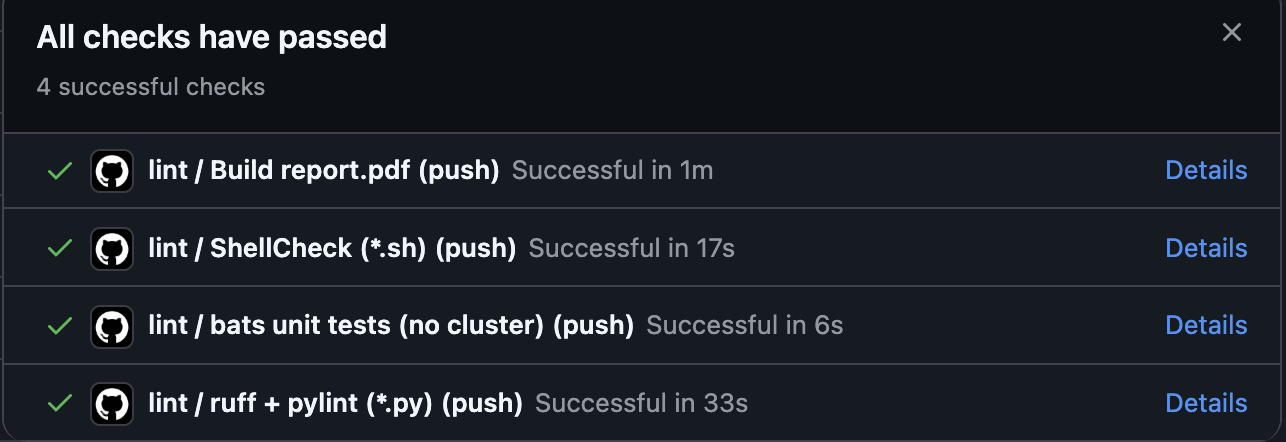
\includegraphics[width=0.78\textwidth]{img/ci_all_passed.png}
\caption{All four jobs green on the current \texttt{main} commit
(\texttt{Build report.pdf} 1m, \texttt{ShellCheck} 17s,
\texttt{bats unit tests} 6s, \texttt{ruff + pylint} 33s). This is the
contract we get on every \texttt{push} and \texttt{pull\_request}.}
\end{figure}

\begin{figure}[H]
\centering
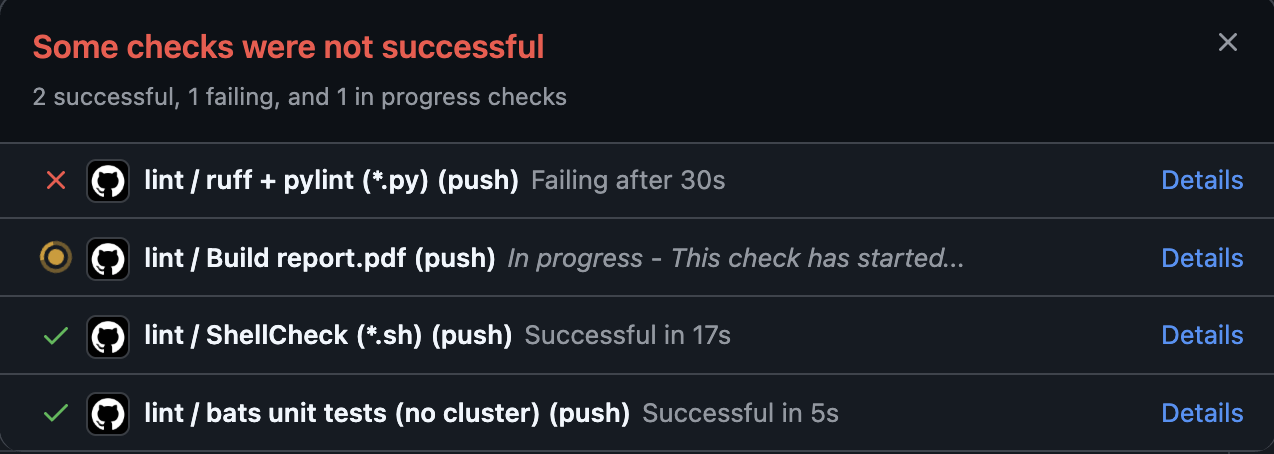
\includegraphics[width=0.78\textwidth]{img/ci_failing.png}
\caption{A failing intermediate run on the same PR --- \texttt{ruff +
pylint} caught a regression and the workflow surfaced it before the
broken commit could be merged. The other three jobs still ran in
parallel, so we got partial feedback in seconds.}
\end{figure}

\subsection{The cluster runner}

\texttt{scripts/run\_tests.sh} is the single entry point for both
unit-style tests (the same ones CI runs) and the cluster smoke suite:

\begin{lstlisting}
# Cloud-safe checks only (what CI runs):
bash scripts/run_tests.sh unit

# Cluster smoke suite (Postgres + Hive + Spark + HDFS):
bash scripts/run_tests.sh smoke

# A single suite by filename prefix:
bash scripts/run_tests.sh smoke 02_postgres
\end{lstlisting}

Every cluster test is gated by \texttt{require\_cmd} and
\texttt{require\_secret} helpers, so the same suite can run anywhere ---
on the cluster it actually validates the warehouse, and on a developer
laptop the cluster tests simply skip with a clear reason.

\begin{figure}[H]
\centering

\includegraphics[width=0.85\textwidth]{img/ci_cluster_passed.png}
\caption{Layer 2 in action --- \texttt{bash scripts/run\_tests.sh unit}
on the cluster from \texttt{team30@hadoop-01}. All 19 unit tests pass:
file-layout invariants, every stage script using \texttt{set -euo
pipefail}, the seven HQL queries present, the \texttt{evaluation.csv}
schema check, and the Random-Forest F1 regression guard.}
\end{figure}

\subsection{What it caught}

A few concrete examples from the project where CI did real work:

\begin{itemize}[leftmargin=2em]
    \item Two \texttt{ml\_models\_training.py} commits introduced
    \texttt{ruff} \texttt{F401} unused-import warnings that nobody
    noticed locally --- caught by the \texttt{python-lint} job on the
    next \texttt{push}.
    \item A broken \texttt{\textbackslash{}cite\{\}} key in
    \texttt{report.tex} slipped through local edits; the
    \texttt{latex-build} job failed loudly on the next push instead of
    leaving us with a quietly mis-rendered PDF.
    \item Several stage scripts were missing \texttt{set -euo pipefail}
    at one point; the \texttt{tests/unit/01\_repo\_structure.bats}
    invariant catches that on \texttt{ubuntu-latest} in under five
    seconds.
\end{itemize}

\subsection{What we shipped}

A reproducible Hadoop pipeline that takes 25M Zeek connection records,
loads them into a Hive warehouse on HDFS, runs seven HiveQL queries on
Tez to surface the structure of the data, trains two Spark ML models with
cross-validation on YARN, and exposes everything in a public Apache
Superset dashboard. Both models clear $F_1 = 0.994$ on the held-out test
set of about 10M rows, with Random Forest at $F_1 = 0.997$. Every
artefact in \texttt{output/} can be regenerated by running
\texttt{main.sh}.

\subsection{How we worked}

The role split worked well. Ivan owned ingestion and the Hive layout;
Kirill owned the Spark feature pipeline and the model grid; Nikita owned
EDA and the dashboard story; Dmitry owned documentation and ran the
re-run checks. The ``one \texttt{main.sh}, every stage idempotent'' rule
was probably the single most useful constraint --- it forced us to
clean up before doing anything, instead of relying on whatever was left
from the last run.

\subsection{What gave us trouble}

\begin{itemize}[leftmargin=2em]
    \item \textbf{Loading the CSVs.} The raw Zeek files use \texttt{-} for
    missing values and write integers as floats (\texttt{1234.0}). The
    Postgres transformation insert had to handle both with
    \texttt{NULLIF} + \texttt{REGEXP\_REPLACE} before casting. One
    missed regex meant a full reload.
    \item \textbf{Partition skew in Hive.} Partitioning by \texttt{label}
    is great for queries but makes one tiny partition (FileDownload,
    3 rows) and four huge ones. Fine for analytical scans, painful for
    Spark shuffles --- we worked around it with
    \texttt{repartition(18)} after the read.
    \item \textbf{Tightening the LR baseline.} An early Logistic
    Regression pass barely beat majority-class until we routed it through
    the same \texttt{ChiSqSelector(fpr=0.1)} block and
    \texttt{StandardScaler(withStd=true)} as Random Forest. The fix
    wasn't more tuning of LR, it was making sure the feature pipeline
    fed it inputs that were comparable in scale and free of the
    high-cardinality one-hot noise --- which lifted F1 from $\approx 0.18$
    to $0.994$.
\end{itemize}

\subsection{What we'd do next}

\begin{enumerate}[leftmargin=2em]
    \item Split by \texttt{capture\_id} instead of by row. Insight 4
    basically tells us we have to.
    \item Add Gradient-Boosted Trees to the grid. With both RF and LR
    already at 0.99+, GBT is the natural next ensemble to try for the
    last percent.
    \item Wire the trained Random Forest into Spark Structured Streaming
    over the same Hive partitions, so it can score new traffic in near
    real time.–
\end{enumerate}

\subsection{Who did what}

\begin{table}[H]
\centering
\small
\renewcommand{\arraystretch}{1.2}
\begin{tabular}{p{4.0cm}p{1.1cm}p{1.1cm}p{1.1cm}p{1.1cm}p{1.0cm}p{2.4cm}}
\toprule
\textbf{Task} & \textbf{Ivan I.} & \textbf{Kirill S.} & \textbf{Nikita Z.} & \textbf{Dmitry T.} & \textbf{Avg hrs} & \textbf{Deliverables} \\
\midrule
Dataset selection \& access            & 25\% & 25\% & 25\% & 25\% & 1  & IoT-23 captures (\href{https://www.kaggle.com/datasets/agungpambudi/network-malware-detection-connection-analysis?select=CTU-IoT-Malware-Capture-44-1conn.log.labeled.csv}{Kaggle Source}) \\
Stage 1 --- PostgreSQL schema \& load  & 100\% & 0\% & 0\% & 0\% & 5  & \texttt{create\_tables.sql}, \texttt{build\_projectdb.py} \\
Stage 1 --- Sqoop \& HDFS warehouse    & 100\% & 0\% &  0\% & 0\% & 8  & \texttt{import\_to\_hdfs.sh} \\
Stage 1 --- Storage benchmark          & 80\% & 0\% &  10\% & 10\% & 4  & \texttt{benchmark\_storage\_*}, CSVs \\
Stage 2 --- Hive warehouse setup       & 90\% & 0\% & 0\% & 10\% & 5  & \texttt{db.hql}, partitioned tables \\
Stage 2 --- 7 EDA queries              & 0\% &  0\% & 90\% & 10\% & 6  & \texttt{q1.hql} \dots \texttt{q7.hql} \\
Stage 2 --- EDA charts \& storytelling & 0\% &  0\% & 80\% & 20\% & 2  & \texttt{output/q*.jpg, q*.csv} \\
Stage 3 --- Feature pipeline           & 0\% & 100\% & 0\% &  0\% & 10 & \texttt{ml\_data\_preparation.py} \\
Stage 3 --- Model training \& CV       & 0\% & 90\% &  5\% &  5\% & 16 & \texttt{ml\_models\_training.py}, \texttt{models/} \\
Stage 3 --- Evaluation                 & 0\% & 80\% & 10\% & 10\% & 7  & \texttt{ml\_evaluation.py}, \texttt{evaluation.csv} \\
Stage 4 --- Superset dashboard         & 10\% & 10\% & 70\% & 10\% & 6  & Public dashboard \\
Pipeline orchestration (\texttt{main.sh}) & 60\% & 20\% & 10\% & 10\% & 2  & \texttt{main.sh}, \texttt{stage*.sh} \\
Repository documentation               & 10\% & 10\% & 10\% & 70\% & 4  & \texttt{README.MD}, \texttt{docs/} \\
Final report (this document)           &  5\% &  5\% & 5\% & 85\% & 8  & \texttt{report/report.pdf} \\
Defence presentation                   & 10\% & 20\% & 30\% & 40\% & 3  & \texttt{presentation/presentation.pdf} \\
QA \& reproducibility checks           & 15\% & 15\% & 15\% & 55\% & 5  & Pipeline re-runs \\
\midrule
\textbf{Total person-hours}            &      &      &      &      & \textbf{92} & \\
\bottomrule
\end{tabular}
\caption{Contribution table. Per-row percentages sum to 100\% across the
four team members; the \emph{Avg hrs} column is the team-wide
person-hours spent on each task.}
\end{table}

\bibliographystyle{plain}
\bibliography{references}
\end{document}
